\chapter{B\'usqueda local}
\label{busqueda}
\epigraph{I don't know what's going on! I don't know where I am! I know I'm
supposed to be looking for someone, but I just can't remember! Can't
remember...}%
{Dory - Finding Nemo}

Finalmente, nos quedan por describir los detalles m\'as relevantes que se
tuvieron en cuenta para implementar el motor combinatorio de \ac{vac-o} y las
interfaces propuestas en la secci\'on~\ref{diseno-motor}. Antes de eso, haremos
un breve repaso por los diferentes paradigmas de b\'usqueda que nos permita
justificar la decisi\'on de utilizar b\'usqueda local.

\section{Paradigmas de b\'usqueda}

La idea fundamental de los algoritmos de b\'usqueda es generar y evaluar
iterativamente soluciones candidatas para un problema determinado. En el caso de
los ``problemas de decisi\'on'', la evaluaci\'on consiste en decidir si la
soluci\'on candidata es una soluci\'on del problema, mientras que para los
``problemas de optimizaci\'on'', la evaluaci\'on consiste t\'ipicamente en
determinar el valor de la funci\'on objetivo para cada soluci\'on candidata.

Generalmente, la evaluaci\'on de las soluciones candidatas depende del problema
y suele ser relativamente f\'acil de implementar\footnote{No es el caso de los
algoritmos para la predicci\'on inversa de estructura secundaria de \ac{RNA},
donde vimos que la evaluaci\'on consiste en realizar la predicci\'on directa y
esto es $\mathcal{O}(N^{3})$.}. Luego, lo que diferencia fundamentalmente a los
distintos algoritmos de b\'usqueda es la forma en que las soluciones candidatas
son generadas. Los paradigmas de b\'usqueda m\'as comunes son:
\begin{itemize}
 \item Perturbativa vs. Constructiva
 \item Local vs. Sistem\'atica
\end{itemize}

Aunque no es necesariamente as\'i, suelen relacionarse la b\'usqueda local con
la b\'usqueda perturbativa y la b\'usqueda sistem\'atica con la b\'usqueda
constructiva.

\subsection{Perturbativa vs. Constructiva}

Las soluciones candidatas de un problema de optimizaci\'on, est\'an compuestas
por las \textit{componentes de la soluci\'on}. Luego, se puede modificar una
soluci\'on candidata para obtener una nueva soluci\'on, cambiando una o varias
de sus componentes. Esto puede ser visto como una \textit{perturbaci\'on} sobre
las soluciones candidatas y por eso se denomina a los algoritmos de b\'usqueda
que utilizan esta forma de generar soluciones candidatas, \textit{algoritmos de
b\'usqueda perturbativa}.

Usualmente en estos algoritmos, la b\'usqueda se realiza sobre el espacio de
soluciones candidatas del problema, pero eventualmente podr\'ia ser \'util
tambi\'en incluir soluciones candidatas parciales en el espacio de b\'usqueda.
Esto es, soluciones candidatas donde una o varias de sus componentes no ha sido
determinada. En ese caso, la tarea consiste en extender las soluciones
candidatas parciales hasta construir soluciones candidatas completas y por eso
se denomina a los algoritmos de b\'usqueda para este tipo de problemas,
\textit{algoritmos de b\'usqueda constructiva}.

\subsection{Local vs. Sistem\'atica}

Otra clasificaci\'on, quiz\'as m\'as com\'un, entre los distintos algoritmos de
b\'usqueda es la distinci\'on entre \textit{b\'usqueda local} y
\textit{b\'usqueda sistem\'atica}. La b\'usqueda sistem\'atica recorre el
espacio de b\'usqueda de una manera sistem\'atica garantizando que
eventualmente, o bien se encuentra una soluci\'on (\'optima), o bien, se tiene
la certeza de que no existe ninguna soluci\'on. Esta propiedad que distingue a
los algoritmos de b\'usqueda sistem\'atica se denomina \textit{completitud}.

Por otro lado, los algoritmos de b\'usqueda local empiezan la b\'usqueda en
alg\'un punto del espacio de b\'usqueda y sucesivamente se mueven de la
soluci\'on actual a una soluci\'on ``vecina'' donde cada movimiento est\'a
determinado solamente por la informaci\'on que brindan la soluci\'on actual y
sus ``vecinos''. Estos algoritmos son t\'ipicamente \textit{incompletos} en el
sentido de que no hay garant\'ia de encontrar una soluci\'on \'optima ni tampoco
se puede determinar con certeza que no exista una soluci\'on. M\'as a\'un, es
posible que los algoritmos eval\'uen mas de una vez la misma soluci\'on o
inclusive queden ``estancados'' en ciertas partes del espacio de b\'usqueda.

\section{?`Por qu\'e usar b\'usqueda local?}

A primera vista, los algoritmos de b\'usqueda local podr\'ian parecer inferiores
a los sistem\'aticos debido a su \textit{incompletitud}, pero esto no es
necesariamente as\'i. Por un lado, una de las propiedades de los algoritmos
sistem\'aticos es la de poder determinar con certeza la existencia o no de una
soluci\'on. En nuestro caso, esto no es relevante ya que el mismo virus atenuado
que se quiere optimizar representa una soluci\'on al problema, por lo que la
existencia de una soluci\'on no est\'a en duda. Adem\'as, los algoritmos
sistem\'aticos y constructivos ponen especial atenci\'on al camino que se
recorre para llegar a una soluci\'on y esto tampoco es de inter\'es en un
problema de optimizaci\'on como el nuestro.

Por otro lado, uno de los problemas que presentan los algoritmos de b\'usqueda
local es determinar el punto en el espacio de b\'usqueda por donde empezar. Una
mala elecci\'on del punto inicial podr\'ia conducir a soluciones sub\'optimas
(m\'inimos o m\'aximos locales), pero esto tampoco ser\'ia un problema en
nuestro caso, ya que el virus atenuado que se quiera optimizar representa
naturalmente un buen punto de inicio por haber demostrado previamente su
efectividad en la pr\'actica.

Por \'ultimo, una de las propiedades deseables en la resoluci\'on de un
problema de optimizaci\'on es que la calidad de las soluciones est\'e
directamente relacionada con el tiempo de ejecuci\'on del algoritmo y esto es
generalmente una propiedad que se da naturalmente en los algoritmos de
b\'usqueda local.

\section{Implementaci\'on}

Como ya mencionamos en la secci\'on~\ref{diseno-motor}, dada la definici\'on
del problema que presentamos en la secci\'on~\ref{formalizacion-prop}, el
objetivo fue capturar la estructura general de los algoritmos de
b\'usqueda local que suelen denominarse de ``mejoramiento iterativo''.

A continuaci\'on presentamos el pseudo c\'odigo para este tipo de algoritmos
asumiendo lo siguiente:

\begin{itemize}
 \item $init$: representa la soluci\'on inicial provista por la extensi\'on.
 \item $s$: representa la soluci\'on actual en cada iteraci\'on.
 \item $explore(s)$: genera el conjunto de soluciones vecinas de $s$.
 \item $select(s, neighbors)$: selecciona una soluci\'on entre las vecinas de
$s$.
 \item $done()$: un predicado que determina cuando terminar la b\'usqueda.
 \item $notify(s')$: notifica a otros objetos la soluci\'on $s'$.
 \item $f(s)$: devuelve la evaluaci\'on de la funci\'on objetivo para $s$.
\end{itemize}

\begin{algorithm}
 \caption{B\'usqueda local}
 \begin{algorithmic}[1]
  \STATE $s \leftarrow init$
  \STATE $neighbors \leftarrow \emptyset$
  \REPEAT
  \STATE $neighbors \leftarrow explore(s)$
  \STATE $s' \leftarrow select(s, neighbors)$  
  \IF{$f(s) \leq f(s')$}
  \STATE $notify(s')$
  \ENDIF
  \STATE $s \leftarrow s'$
  \UNTIL{$done()$}
 \end{algorithmic}
\end{algorithm}

Claramente, la implementaci\'on de los procedimientos $explore$ y $select$
ser\'an determinantes en este algoritmo y sobre ellos profundizaremos a
continuaci\'on. Por otro lado, el criterio de terminaci\'on estar\'a
relacionado con el n\'umero total de iteraciones y con el n\'umero de
iteraciones que pasaron desde la mejor soluci\'on encontrada. Ambos
par\'ametros, provistos por la extensi\'on.

Se puede trazar una analog\'ia entre este tipo de algoritmos y buscar el
m\'aximo de una funci\'on. El algoritmo empieza en alg\'un punto de la
funci\'on, que en nuestro caso ser\'a el virus atenuado que se pretende
optimizar y luego en cada iteraci\'on, el algoritmo debe ``moverse'' de la
soluci\'on actual a la siguiente con el objetivo de maximizar la funci\'on de
evaluaci\'on.
\begin{figure}
 \centering
 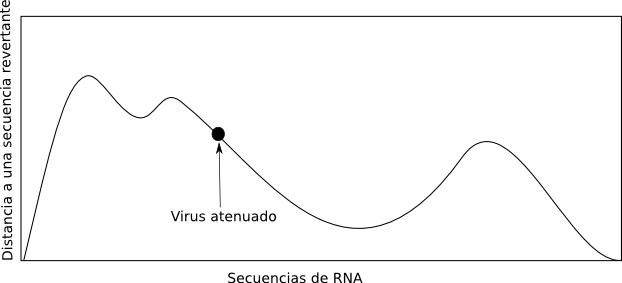
\includegraphics[scale=.75]{hillclimbing.png}
 \caption{B\'usqueda local por mejoramiento iterativo}
 \label{hillclimbing}
\end{figure}


\subsection{El vecindario}

El concepto de ``vecindario'' de una soluci\'on es crucial para determinar los
posibles movimientos de una soluci\'on a la siguiente. Esto puede ser visto
b\'asicamente como una relaci\'on entre soluciones, y si decimos que
$\mathcal{S}$ es el espacio de soluciones, entonces un vecindario ser\'a una
relaci\'on $\mathcal{N} \subseteq \mathcal{S} \times \mathcal{S}$.

La interfaz propuesta en la secci\'on~\ref{diseno-motor} para representar esta
relaci\'on entre soluciones fue \textbf{INeighborhood} y cuya principal
responsabilidad es la de \textit{explorar} el vecindario de una soluci\'on dada.
Es decir, para una soluci\'on $s$, generar el conjunto de soluciones vecinas
$\mathcal{N}(s)$. 

Para implementar esta interfaz, se propuso una variante de un tipo de
vecindarios que se conoce usualmente como \textbf{k-opt}, en donde dos
soluciones son vecinas si difieren en a lo sumo $k$ componentes de la
soluci\'on. Recordemos que en nuestro caso, las componentes de la soluci\'on son
esencialmente las regiones combinatorias representadas por la interfaz
\textbf{ICombinatoryRegion} y cuya principal responsabilidad es la de generar
las variantes de la regi\'on combinatoria que satisfacen las restricciones
impuestas. Luego, la definici\'on de vecindario que se propuso fue la siguiente:

\begin{definition}
 Para $\mathcal{S}$ el espacio de soluciones, $N$ regiones combinatorias y
$m>0$, sea $\mathcal{N} \subseteq \mathcal{S} \times \mathcal{S}$ tal que,
para $s, s' \in \mathcal{S}$ el par $(s,s') \in \mathcal{N}$ si se satisfacen:
\begin{itemize}
 \item $s'$ difiere de $s$ en a lo sumo una regi\'on combinatoria
(\textbf{1-opt}).
 \item Si $s'$ difiere de $s$ en la regi\'on $r$, entonces se generaron a lo
sumo $m$ variantes de la regi\'on combinatoria $r$.
 \item Si $v_{1}, \dots, v_{N}$ son las variantes a cada regi\'on combinatoria
en la soluci\'on $s'$, entonces $\prod_{i=1}^{N} eval(v_{i}) \ge umbral$.
\end{itemize}
\end{definition}

Algunas alternativas inmediatas que surgen a esta definici\'on son:
\begin{itemize}
 \item Permitir que la soluciones vecinas difieran en m\'as de una regi\'on
combinatoria.
 \item Hacer que el n\'umero $m$ de variantes generadas para cada regi\'on sea
variable en el tiempo de forma tal de expandir el vecindario a medida que avanza
la b\'usqueda.
\end{itemize}

\subsection{La estrategia}

Una vez que se generan las soluciones vecinas de la soluci\'on actual, se
necesita alg\'un criterio para \textit{seleccionar} una entre todas ellas. Esto
es lo que se propuso representar con la interfaz \textbf{IStrategy}.
B\'asicamente, las implementaciones de esta interfaz determinan el criterio de
selecci\'on y representan las principales diferencias entre los distintos
algoritmos de b\'usqueda local. A continuaci\'on veremos brevemente las tres
estrategias implementadas. Supongamos como antes, $\mathcal{S}$ es el espacio de
soluciones, $\mathcal{N} \subseteq \mathcal{S} \times \mathcal{S}$ la relaci\'on
que define el vecindario, $f: \mathcal{S} \rightarrow \mathbb{R}$ la funci\'on
objetivo y $s \in \mathcal{S}$ la soluci\'on actual.

\subsubsection{\textit{Best Improvement}}

Esta estrategia consiste en seleccionar una soluci\'on $s' \in \mathcal{N}(s)$
de forma tal que $f(s) \leq f(s')$ y adem\'as $f(s') = \max_{c \in
\mathcal{N}(s)} f(c)$. Notar que, por un lado podr\'ia existir mas de una
soluci\'on que maximice la funci\'on $f$ para el conjunto $\mathcal{N}(s)$, en
cuyo caso se seleccionar\'a alguna de ellas. Por otro lado, esta estrategia
implica generar y evaluar todas las soluciones vecinas de $s$, lo que
podr\'ia ser eventualmente costoso dependiendo del tama\~no del conjunto
$\mathcal{N}(s)$.

\subsubsection{\textit{First Improvement}}

A diferencia de \textit{Best Improvement}, esta estrategia supone que los
vecinos de $s$ son generados en alg\'un orden. Luego, en lugar de
\textit{explorar} todo el vecindario para luego seleccionar la
siguiente soluci\'on, se selecciona la primer soluci\'on $s' \in
\mathcal{N}(s)$ tal que $f(s) \leq f(s')$. Obviamente, esto implica un ahorro en
el sentido de que no se generan y eval\'uan todas las soluciones vecinas de $s$,
pero al mismo tiempo se corre el riesgo de descartar soluciones mejores a la
seleccionada.

\subsubsection{\textit{Simulated Annealing}}

Esta estrategia marca una diferencia importante con las anteriores como es la
posibilidad de seleccionar soluciones que \textbf{no} mejoran la soluci\'on
actual, pero que eventualmente podr\'ian conducir a mejores soluciones. Esto es
fundamentalmente para ``escapar'' de los m\'aximos locales que podr\'ian existir
en el espacio de soluciones. 

Por un lado, para seleccionar una soluci\'on peor que la actual, se debe tener
en cuenta la diferencia entre sus respectivas evaluaciones, a mayor diferencia,
menor deber\'ia ser la probabilidad de seleccionarla. Adem\'as, se supone que a
medida que avanza la b\'usqueda, la calidad de las soluciones deber\'ia
incrementarse, por lo tanto, la probabilidad de seleccionar una soluci\'on peor
que la actual debe ser cada vez menor.

En definitiva, la estrategia consiste en seleccionar aleatoriamente una
soluci\'on $s' \in \mathcal{N}(s)$ y luego decidir si $s'$ es aceptada o no.
Si $f(s) \leq f(s')$, $s'$ se acepta autom\'aticamente. Pero si $f(s) > f(s')$,
entonces $s'$ se acepta con probabilidad $exp(\frac{f(s') - f(s)}{T})$. Donde $T
> 0$, es un par\'ametro que permite modular la probabilidad de aceptaci\'on a
medida que avanza la b\'usqueda. Luego, cada alg\'un n\'umero prefijado de
iteraciones, se actualiza el valor de $T$ haciendo $T = T\times \alpha$ para $0
< \alpha < 1$.

